\section{对流}\label{sec:2-6}

在图 \ref{fig:2-14} 的实验里,如果我们不是给试管上部的水加热,而是给试管底部的水加热,整个试管中的水都会很快热起来。
同样,在图 \ref{fig:2-15} 的实验里,如果让试管的口向上,给试管底部的空气加热,手指也会很快觉得热了。
既然水和空气都是热的不良导体,那么,在上述情况下,热是怎样传递的呢?

\begin{wrapfigure}[17]{r}{6cm}
    \centering
    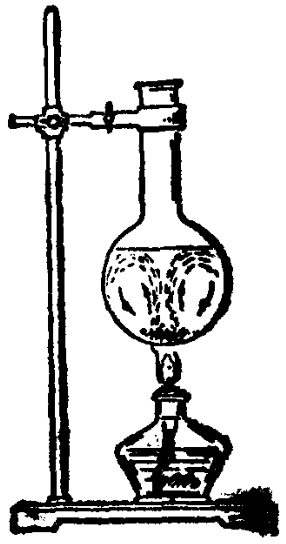
\includegraphics[width=5cm]{../pic/czwl2-ch2-16}
    \caption{水的对流}\label{fig:2-16}
\end{wrapfigure}


如图 \ref{fig:2-16} 所示,把装有冷水的烧瓶悬空架在铁架台上。
水静止后,投入一些高锰酸钾的晶粒,使它沉到瓶底。用酒精灯的小火在烧瓶下面对准晶粒加热。
我们会看到,晶粒周围的紫红色溶液向上升起形成一股股细流,然后又沿瓶的边缘流回瓶底,不一会,
整瓶水都成了紫红色的高锰酸钾溶液。高锰酸钾溶液的流动过程清楚地表示出热传递的情况。
晶粒处的水受热膨胀、密度减小而上升,旁边密度较大的冷水就流过来填补。
流到晶粒处的冷水被加热后又上升,旁边的冷水又流过来填补。这样,水就循环流动起来。
最后,整个烧瓶里的水都变热了。在这里,热是靠水的流动来传递的。

空气的流动也可以传热。例如,冬季用火炉或暖汽片取暖就是靠空气的流动。
火炉或暖汽片使整个屋子空气变暖的过程,同学们可以参照液体流动传热的情况来自己分析。

靠液体或者气体的流动来传递热的方式叫做\textbf{对流}。

根据上面关于对流的讨论知道,要使整个容器中的液体(或气体)的温度很快升高,
应该从下方来加执,因为这样可以形成对流。
我们烧开水的时候,把水壶放在炉火的上面,就是这个道理。

要使整个容器中的液体(或气体)的温度很快降低,应该从上方来冷却,
同样也是因为这样可以形成对流。我们用冰块来冷藏食物的时候,
把冰块放在食物上面比放在下面效果好,就是这个道理。

学过传导和对流以后,我们不难看出它们的区别:
传导是热沿着物体传递的,物质并不流动;
对流是靠物质的流动来传热的。
所以对流是液体、气体特有的传热的方式。



\section*{阅读材料:水的反常膨胀}

在北方,冬季湖水结冰总是从湖面开始,这种现象你不感到奇怪吗?
学过对流以后,爱动脑筋的学生是会感到奇怪的。
因为寒冬降临,冷空气从上方来冷却湖水,假如水总是热胀冷缩,湖水会形成对流,
使全部湖水都降到 $0\celsius$ 而结冰。实际情况为什么不是这样呢?

原来,水的热膨胀有它的特殊性。水在 $4\celsius$ 以上,跟一般的物体一样,是热胀冷缩的,
但是在 $0\celsius$ 到 $4\celsius$ 之间却是热缩冷胀的。
因此,$4\celsius$ 的水无论温升高或降低,体积都要增,密庹都要减小。
就是说,水在 $4\celsius$ 的时候,密度最大。

\begin{figure}[htbp]
    \centering
    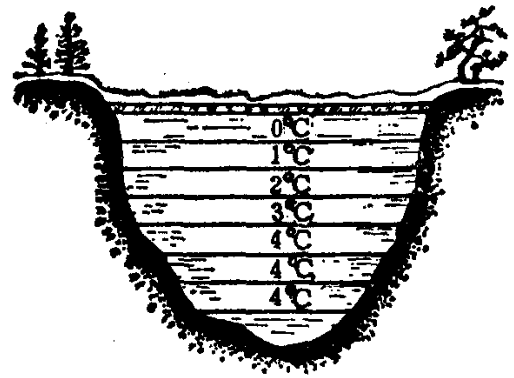
\includegraphics[width=0.3\textwidth]{../pic/czwl2-ch2-17}
    \caption{表面结了冰的湖水的温度}\label{fig:2-17}
\end{figure}

现在我们分析湖水结冰的情况。气温下降时,湖面的水温度也要降低。
在 $4\celsius$ 以上时,由于热胀冷缩,湖面温度较低的水,密度较大要下沉;底部温度较高的水,密度较小,要上升。
这面,湖面较冷的水和底部较暖的水,它们的温度很快就会达到一致了。
湖面的水,当温度降低到 $4\celsius$ 以下时,由于热缩冷胀,密度反而减小,不再下沉,就不再形成对流了。
因此,湖面冷却到结了冰,而底部水的温度仍然可以保持 $4\celsius$ (图 \ref{fig:2-17}),鱼类仍旧可以自由自在地游来游去。



\section*{小实验}

照图 \ref{fig:2-18} 甲那样,在一张厚的图画纸上画线。沿实线剪开,再沿虚线折起,做成一个叶轮。
用细线把叶轮悬起来,在它的下方点燃一根火柴,叶轮就转起来(图乙)。
你自己动手做一做,并说明叶轮为什么会转。

\begin{figure}[htbp]
    \centering
    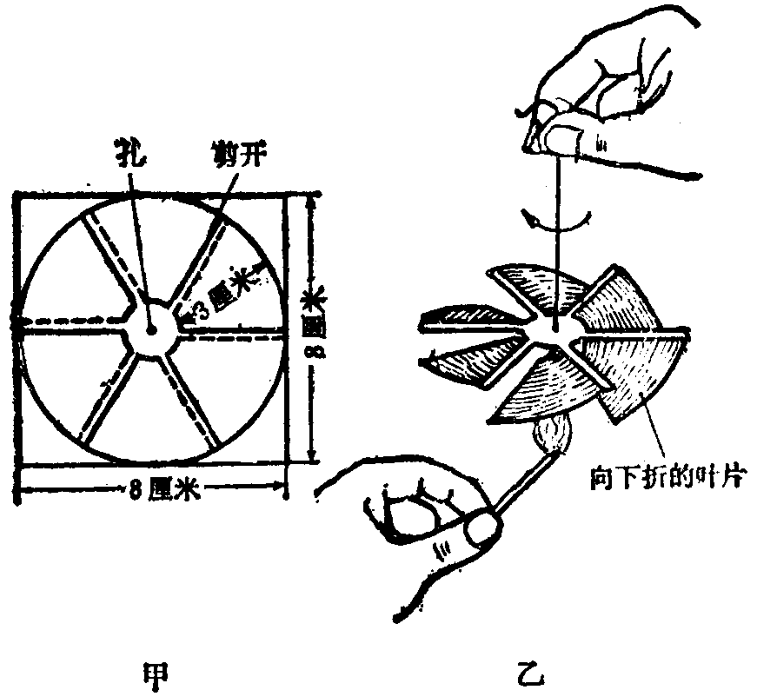
\includegraphics[width=0.5\textwidth]{../pic/czwl2-ch2-18}
    \caption{}\label{fig:2-18}
\end{figure}


